

\documentclass[12pt, a4paper]{article}

% Set the document margins for [A4 paper; and, left, right, top, and bottom margins; the text to footer gap; and include the footer in the main body of the text (so page numbers leave space equal to the bottom value just specified)]
\usepackage[a4paper, left=2.5cm, right=2cm, top=2cm, bottom=2cm, footskip=1.5cm, includefoot]{geometry}

\usepackage{natbib}
\usepackage{graphicx}
\usepackage{booktabs}
\usepackage[hidelinks]{hyperref} % to insert a web link
\usepackage{amsfonts} % to get blackboard font

\usepackage{listings} % to get code blocks
\usepackage{xcolor}
\definecolor{codegreen}{rgb}{0,0.6,0}
\definecolor{codegray}{rgb}{0.5,0.5,0.5}
\definecolor{codepurple}{rgb}{0.58,0,0.82}
\definecolor{backcolour}{rgb}{0.9,0.9,0.9}
\lstdefinestyle{mystyle}{
    backgroundcolor=\color{backcolour},   
    commentstyle=\color{codegreen},
    keywordstyle=\color{magenta},
    numberstyle=\tiny\color{codegray},
    stringstyle=\color{codepurple},
    basicstyle=\ttfamily\footnotesize,
    breakatwhitespace=false,         
    breaklines=true,                 
    captionpos=b,                    
    keepspaces=true,                 
    numbers=left,                    
    numbersep=5pt,                  
    showspaces=false,                
    showstringspaces=false,
    showtabs=false,                  
    tabsize=2
}
\lstset{style=mystyle}


\begin{document}


\title{\texttt{compGeometeR}: an \texttt{R} package for computational geometry}

\author{Thomas R. Etherington  \\
	Manaaki Whenua -- Landcare Research  \\
	\and 
	O. Pascal Omondiagbe \\
	Manaaki Whenua -- Landcare Research \\
	}



\date{\today}



\maketitle


\begin{abstract}

Computational geometry algorithms and data structures are widely applied across numerous scientific domains, and there a variety of \texttt{R} packages that apply computational geometry.  However, these packages often work in specific numbers of dimensions, have incompatible data structures, and include additional non-computational geometry functionality that can be domain specific.  Our objective in developing the \texttt{compGeometeR} package is to produce a systematic implementation of the most commonly used computational geometry algorithms so that they can be easily integrated into domain specific scientific workflows.  We briefly explain the algorithms available in \texttt{compGeometeR}, and identify priorities for future development.

\begin{center}
\textbf{Keywords}: alpha complex, alpha shape, convex hull, convex layers, Delaunay triangulation, digital, discrete.
\end{center}

\end{abstract}

\section{Introduction}

Computational geometry seeks to develop algorithms and data structures for geometric objects, and the results are widely applied across numerous scientific domains \citep{de-berg-2008}.  Given the importance of computational geometry it is no surprise that within the \texttt{R} computing ecosystem there are a variety of options for applying various computational geometry algorithms.  However, these packages often work in specific numbers of dimensions, have incompatible data structures, and include additional non-computational geometry functionality that can be domain specific.

Our objective in developing the \texttt{compGeometeR} package is to produce a systematic implementation of some of the most commonly used computational geometry algorithms across various of branches of geometry so that they can be easily integrated into domain specific scientific workflows.

\section{Algorithms}

There are a variety of computational geometry algorithms available in \texttt{compGeometeR}, some of which are replicated in other \texttt{R} packages.  By documenting these differences (Table \ref{tab:r-options}) we hope to help potential users to assess if \texttt{compGeometeR} is the best option for their needs as there may be other options that are more suitable.

The functions of \texttt{compGeometeR} interconnect and build upon one another, but it is important to recognise that virtually all of the \texttt{compGeometeR} functions are  dependent on computational geometry foundations provided by the \texttt{Qhull} C++ interface software \citep{barber-1996}.

% The following table uses formatting fucntions of the booktabs package: https://texdoc.org/serve/booktabs/0
\begin{table}
\small
\centering
\caption{Computational geometry software options in \texttt{R}.  For each computational geometry function, the \texttt{R} software (and version) that can apply this algorithm is noted by reference to the number of dimensions in which the algorithm will work.}
\begin{tabular}{l c c c c c c c c}
  \toprule

   & \rotatebox{90}{\texttt{compGeometeR} (1.0.0)}
   & \rotatebox{90}{\texttt{R} (3.5.3)}
   & \rotatebox{90}{\texttt{alphahull} (2.2)}
   & \rotatebox{90}{\texttt{alphashape3d} (1.3.1)}
   & \rotatebox{90}{\texttt{deldir} (0.1-25)}
   & \rotatebox{90}{\texttt{geometry} (0.4.5)}
   & \rotatebox{90}{\texttt{spatstat} (1.63-3)}
   & \rotatebox{90}{\texttt{tripack} (1.3-9.1)} \\

  \cmidrule{1-9} 
  Discrete geometry		&     &   &     &   &   &     &   &   \\
  \cmidrule{1-9} 
  Alpha complex				& $n$ &   &     &   &   &     &   &   \\
  Alpha shape				&     &   &  2  & 3 &   &     &   &   \\
  Convex hull  				& $n$ & 2 &     &   &   & $n$ & 2 & 2 \\
  Convex layers				& $n$ &   &     &   &   &     &   &   \\
  Delaunay triangulation	& $n$ &   &  2  &   & 2 & $n$ & 2 & 2 \\
  Voronoi diagram			&     &   &  2  &   & 2 & $n$ & 2 & 2 \\
  
  \cmidrule{1-9} 
  Digital geometry			&     &   &     &   &   &     &   &   \\
  \cmidrule{1-9} 
  Alpha complex				& $n$ &   &     &   &   &     &   &   \\
  Alpha shape				& $n$ &   &     &   &   &     &   &   \\
  Convex hull  				& $n$ &   &     &   &   &     &   &   \\
  \bottomrule
\end{tabular}
\label{tab:r-options}
\end{table}

\begin{figure}[ht]
\centering
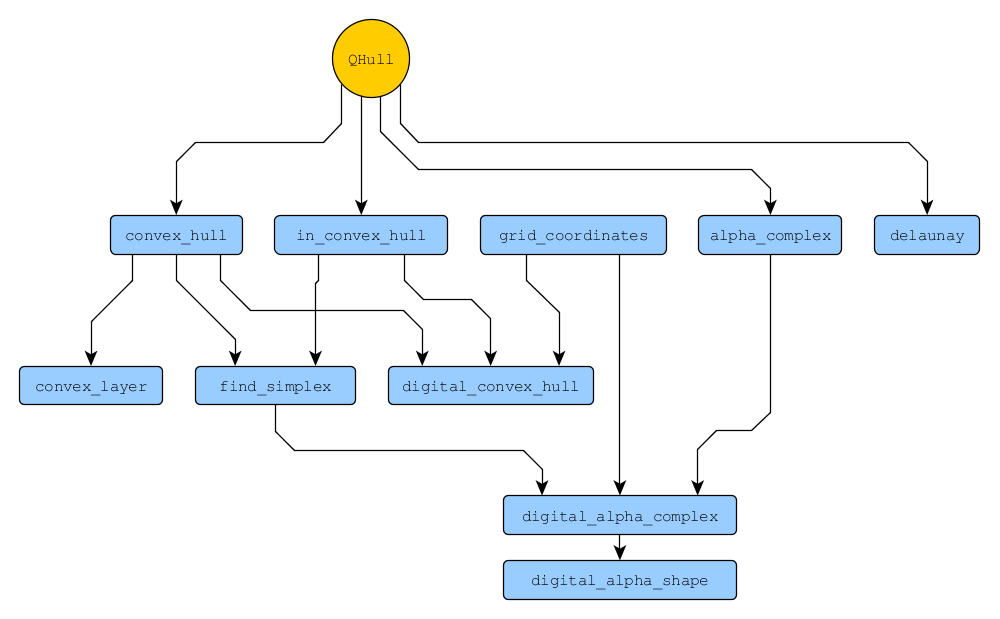
\includegraphics[width=15cm]{figures/software-structure/software-structure.png}
\caption{Connections and dependencies of the \texttt{compGeometeR} functions.}
\label{fig:software-structure}
\end{figure}

\subsection{Discrete geometry}
% see: https://en.wikipedia.org/wiki/Discrete_geometry

Discrete geometry studies the shapes and interactions between sets of discrete objects such as points, lines, circles, and polygons in 2-dimensional space.  All of the discrete computational geometry algorithms in \texttt{compGeometeR} take as an input a set of points $P$ in $n$-dimensional Euclidean space $\mathbb{R}^n$.

A convex hull \citep{barber-1996} defines the smallest subset of $\mathbb{R}^n$ that contains $P$ and for which the subset is convex so any two points within the convex hull can be connected by a straight line also contained by the convex hull (Figure \ref{fig:discrete-algorithms}a).  As an example of the simplicity of \texttt{compGeometeR} a convex hull can be generated and visualised with minimal code (Listing \ref{code:discrete-convex-hull-code}).

\begin{lstlisting}[language=R, caption=Example \texttt{R} code to create a discrete convex hull with \texttt{compGeometeR}, label={code:discrete-convex-hull-code}]
library(compGeometeR)
# Generate point data
set.seed(2) # to reproduce figure exactly
x = rgamma(n = 20, shape = 3, scale = 2)
y = rnorm(n = 20, mean = 10, sd = 2)
p = cbind(x, y)
# Create convex hull
ch = convex_hull(p)
# Plot point data and convex hull
plot(x, y, yaxt="n", xaxt="n", xlab="", ylab = "", pch=16, cex=0.75)
polygon(ch$hull_vertices, col="orange", border="firebrick")
points(p, pch=16, cex=0.75)
\end{lstlisting}

Convex layers were first presented by \cite{huber-1972} and \cite{barnett-1976} who both gave unreferenced credit for this idea to Tukey.  Convex layers are a nested sequence of convex hulls produced by repeating the process of constructing a convex hull for $P$ and then removing the points forming the vertices of the convex hull from $P$ before producing the next convex layer.  The first convex layer is equivalent to the convex hull, with each successive convex layer representing ever smaller region of space (Figure \ref{fig:discrete-algorithms}b).

The Delaunay triangulation \citep{delaunay-1934} produces a set of simplices (triangles in 2-dimensions or tetrahedrons in 3-dimensions) for which no point in $P$ is inside the the circumhypersphere (a circle in 2-dimensions or a sphere in 3-dimensions) of each simplex (Figure \ref{fig:discrete-algorithms}c).

The alpha complex \citep{edelsbrunner-1994} is a subset of the Delaunay triangulation that contains only those simplices for whose circumhypersphere radius is smaller than a specified $\alpha$ parameter value ranging $0 < \alpha < \infty$ (Figure \ref{fig:discrete-algorithms}d).  The related alpha shape would be a polytope that combines all of the simplices in an alpha complex \citep{edelsbrunner-1994}.

\begin{figure}[ht]
\centering
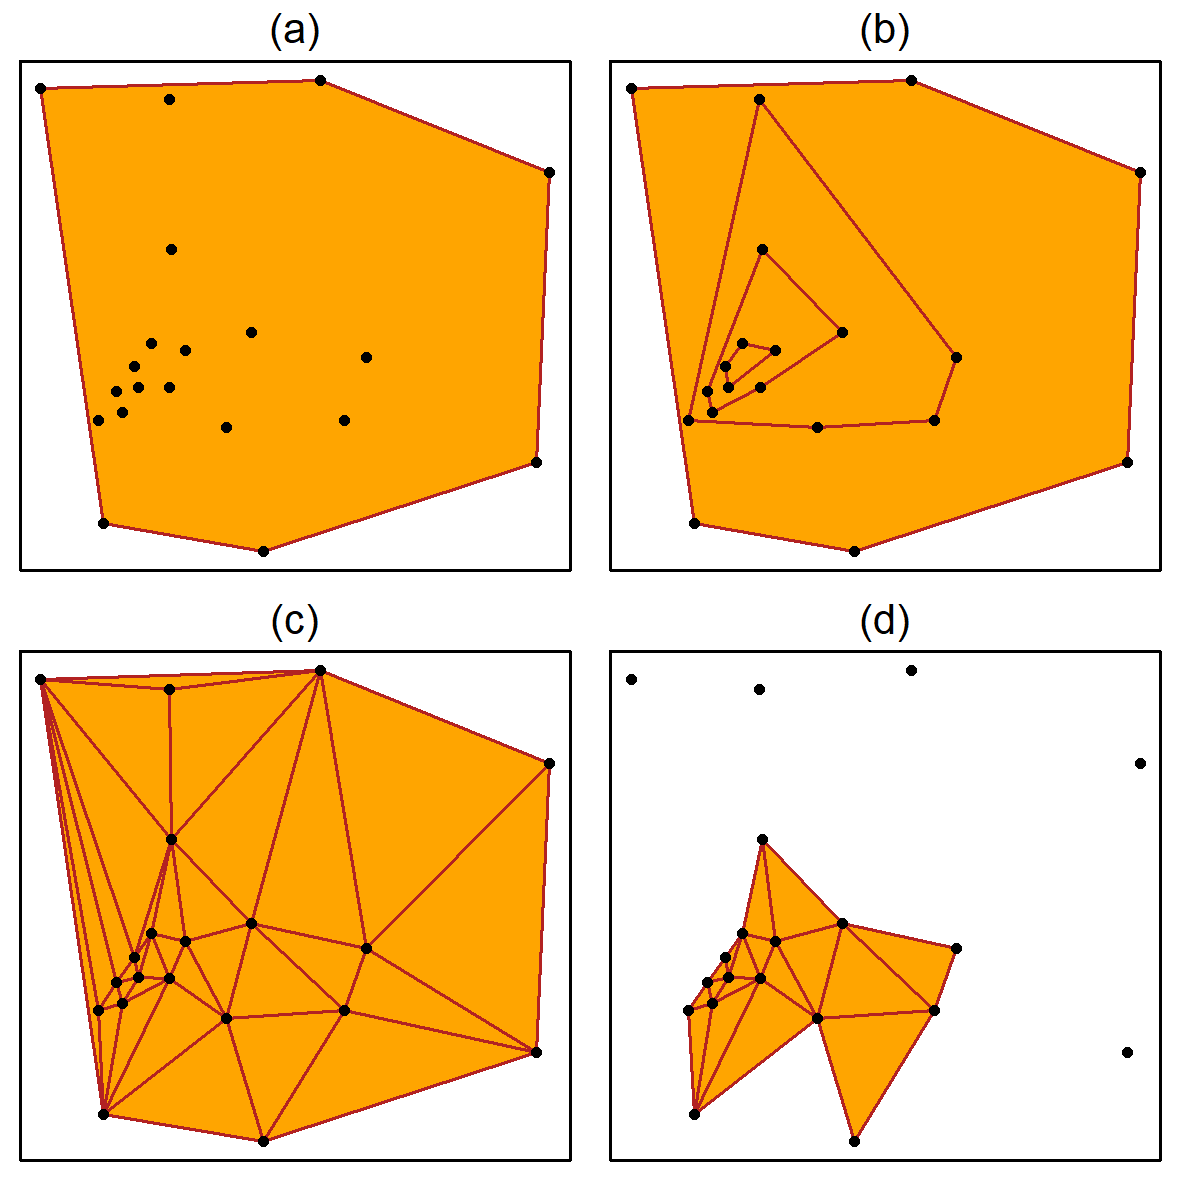
\includegraphics{figures/discrete-algorithms/discrete-algorithms.png}
\caption{Two-dimensional examples of discrete geometry algorithms currently available in \texttt{compGeometeR}. (a) Convex hull, (b) convex layers, (c) Delaunay triangulation, and (d) alpha complex.}
\label{fig:discrete-algorithms}
\end{figure}

\subsection{Digital geometry}
% see: https://en.wikipedia.org/wiki/Digital_geometry

Digital geometry is a branch of geometry that studies the geometric properties of a grid (or lattice) of points in Euclidean space, and usually involves the digitisation of discrete lines and regions \citep{rosenfeld-1989}.  Digitisation occurs by representing Euclidean space $\mathbb{R}^n$ as a a rectangular orthogonal grid $\mathbb{G}^n$.  The elements of $\mathbb{G}^2$ are called pixels, and the elements of $\mathbb{G}^3$ are called voxels, and each element in $\mathbb{G}^n$ has a grid coordinate for its centre \citep{klette-2004} and a value that denotes if the element belongs to a digitised geometric object, or when required, which part of the digitised geometric object.  \texttt{compGeometeR} has implemented digital versions of the convex hull (Figure \ref{fig:digital-algorithms}a), alpha complex (Figure \ref{fig:digital-algorithms}b), and alpha shape (Figure \ref{fig:digital-algorithms}c) that are unique functions amongst \texttt{R} software (Table \ref{tab:r-options}).

The code required for digital versions of the discrete algorithms is no more complicated, and simply requires addtional parameters to define the extent and resolution of $\mathbb{G}^n$.  For example, the code required for a digital convex hull (Listing \ref{code:digital-convex-hull-code}) does not differ much from that required for a discrete convex hull (Listing \ref{code:discrete-convex-hull-code}).

\begin{lstlisting}[language=R, caption=Example \texttt{R} code to create a digital convex hull with \texttt{compGeometeR}, label={code:digital-convex-hull-code}]
library(compGeometeR)
# Generate point data
set.seed(2) # to reproduce figure exactly
x = rgamma(n = 20, shape = 3, scale = 2)
y = rnorm(n = 20, mean = 10, sd = 2)
p = cbind(x, y)
# Create digital convex hull
d_ch = digital_convex_hull(p, mins=c(0,5), maxs=c(15,15), spacings = c(0.05,0.05))
# Plot point data and digital convex hull
image(x=d_ch[[3]][[1]], y=d_ch[[3]][[2]], z=d_ch[[1]], 
      yaxt="n", xaxt="n", xlab="", ylab = "", col=c("white", "orange"))
points(p, pch=16, cex=0.75)
\end{lstlisting}

\begin{figure}[ht]
\centering
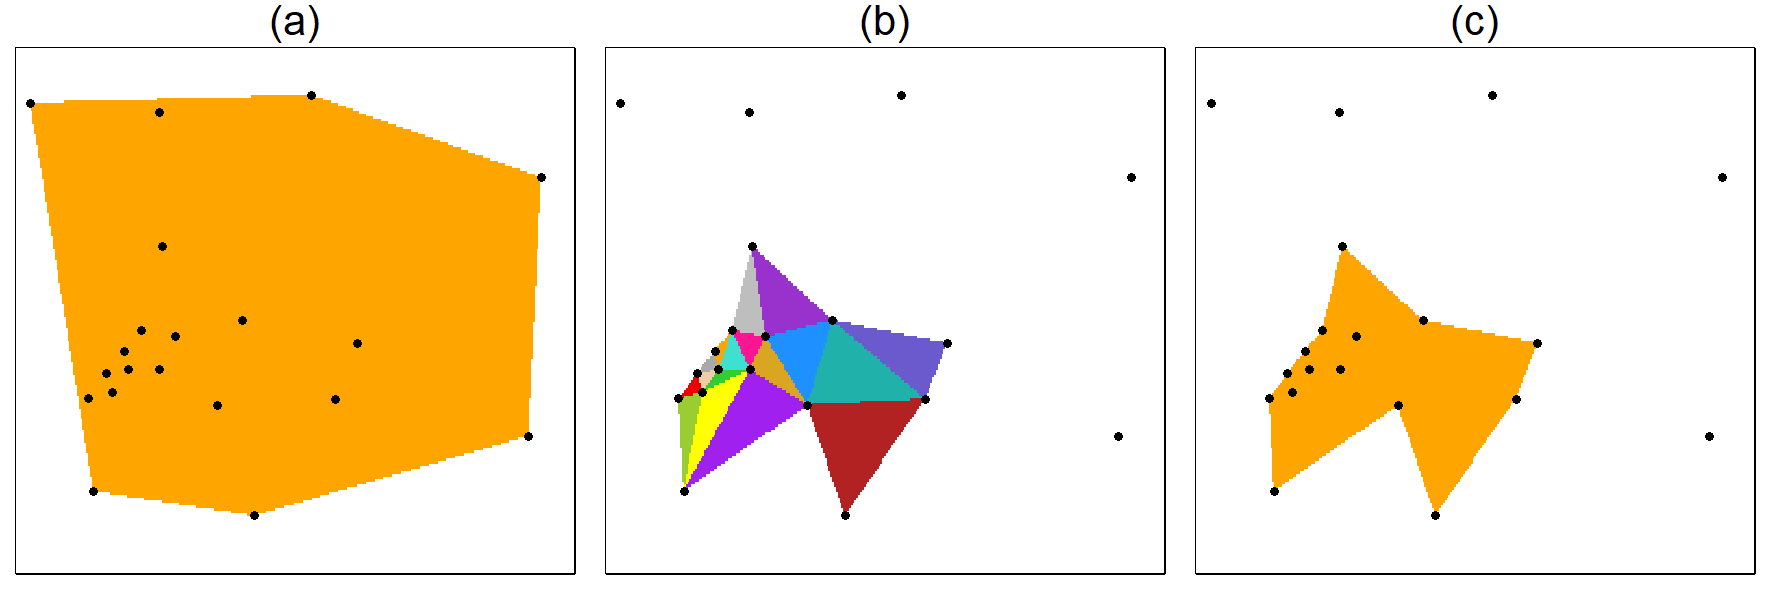
\includegraphics{figures/digital-algorithms/digital-algorithms.png}
\caption{Two-dimensional examples of digital geometry algorithms currently available in \texttt{compGeometeR}. (a) Convex hull, (b) alpha complex, and (c) alpha shape.}
\label{fig:digital-algorithms}
\end{figure}

\section{Future work}

\texttt{compGeometeR} is very much a work in progress, and while there is sufficient functionality for it to be of wide use in the computational sciences, there is some functionality that has been identified as being particularly useful for future development.

The Voronoi diagram \citep{voronoi-1908, okabe-2000} partitions $n$-dimensional space into a set of polytopes for which each polytope delineates the region of $n$-dimensional space that is closest to each point in $P$.  The Voronoi diagram would be an obvious addition for the discrete geometry algorithms given its wide implementation in other R geometry packages (Table \ref{tab:r-options}).

As well as expanding the number of discrete geometry algorithms, and implementing more discrete algorithms in digital form, there are other kinds of computational geometry algorithms that we think would be of particular value.

There are a variety of useful graph structures that can be produced based on geometric principles.  For example, the Delaunay triangulation \citep{delaunay-1934} can also be represented as a graph structure, and for which there are several useful subgraphs such as the Gabriel graph \citep{gabriel-1969}, Urquhart graph \citep{urquhart-1980}, and relative neighbourhood graph \citep{toussaint-1980}.

In some contexts it will be important to recognise that there is uncertainty in the position of points in space and the parameters defining a given algorithm.  In such situations it may be helpful to adopt fuzzy geometry \citep{rosenfeld-1998} view in which, foe example, memberships of points in space are not crisp being either 0 or 1, but rather are fuzzy on a scale from 0 to 1.  Creating fuzzy versions of the \texttt{compGeometeR} algorithms could result in very useful functionality where quantifying uncertainty of any computational geometry is important.  The existing digital geometric algorithms could be easily extended to fuzzy forms as all that is required is to assign a membership value to each pixel \citep{klette-2004}.

All the algorithms in \texttt{compGeometeR} work in Euclidean space, but computational geometry algorithms can also be usefully applied in spherical or hyperbolic space \citep{gowers-2003}.  For example, the Fortran \texttt{STRIPACK} software \citep{renka-1997} could be wrapped by R to provide functionality to compute Delaunay triangulations and Voronoi diagrams on the surface of a sphere.

\section{Software availability}

\texttt{compGeometeR} is open source software made available under a General Public License license. Installation instructions can be found at the GitHub repository \url{https://github.com/manaakiwhenua/compGeometeR}.

We are also developing a cookbook of examples of \texttt{compGeometeR} use via the GitHub repository wiki \url{https://github.com/manaakiwhenua/compGeometeR/wiki}.

\section{Acknowledgements}

This research was funded by the New Zealand Ministry of Business, Innovation and Employment via the Beyond Myrtle Rust (\#C09X1806) and Winning Against Wildings research programmes, with additional internal investment by Manaaki Whenua -- Landcare Research

\bibliographystyle{landscapeecol}
\bibliography{references}


\end{document}